\section{Question 5}
\paragraph{(a)} Transfer function is given by
\begin{equation}
T(s) = \frac{\theta}{\theta_d}= \frac{k_p 65}{s^2 + (37+65 k_v)s + k_p 65}
\end{equation}

\paragraph{(b)} Natural frequency $w_n=\sqrt{k_p 65}$, damping ratio $\zeta=\frac{37+65 k_v}{2\sqrt{k_p 65}}$. Hence, increase $k_p$ increases value of $w_n$ (thus, reduce rise time ($t_r$)), reduce value of $\zeta$ (thus, increase overshoot ($\%PO$)) and reduce $w_n$; whereas  increase value $k_v$ increases value of $\zeta$ (thus, reduce overshoot ($\%PO$)), and does not affect $w_n$ and rise time ($t_s$).


\paragraph{(d)} Considering a desired damping ratio ($\zeta$) equal to $0.5$ and rise time ($t_r$) equal to $1$ second (natural frequency equal to $2.41$ $\mathrm{\frac{rad}{s}}$). Hence, desired poles are
\begin{align*}
	p_1 &= -1.214 + 2.0917 i, \\
	p_2 &= -1.214 - 2.0917 i.
\end{align*}

Then, control gains should be $k_p =0.09$ and $k_v =-0.532$. Finally, step response of close-loop system with proportional-velocity control method is shown in Figure~\ref{fig:q5_step_response_T}.

\begin{figure}[h!]
	\centering
	\includegraphics{images/q5_step_response_T.eps}
	\caption{Step response of close-loop system (T) with proportional-velocity control method ($k_p=0.09$ and $k_v=-0.532$).}
	\label{fig:q5_step_response_T}
\end{figure}

\paragraph{(e)} Close loop system with proportional-integral control method is given by
\begin{equation}
	T(s) = \frac{65 k_p s + 65 k_i}{s^3 + 37 s^2 + 65 k_p s + 65 k_i},
\end{equation}
\noindent where $k_p$, $k_i$ is proportional and integral gains. Figure \ref{fig:q5_bode_T_PI} shows root-locus of close-loop system with different configurations of  proportional-integral control method. On one hand, Figure \ref{fig:q5_bode_a} describes root-locus when integral and proportional gains have the relation $10:1$. In this figure, the three poles are located in left half-plane; thus, close-loop system is stable with a regular overshoot and setting time. On the other hand, Figure \ref{fig:q5_bode_b} describes root-locus when integral and proportional gains have the relation $1:10$. In this figure, two poles are complex and one pole is close to  $0$; thus, close-loop system is stable and could present a behavior without oscillations with adequate control gains ($k_p, k_i$). Finally, Figure show the step response of close-loop system with both cases of relation between integral and proportional gain (the control gains are indicated in data box of  Figure \ref{fig:q5_bode_T_PI}).

\begin{figure}
	\centering
	\subfloat[]{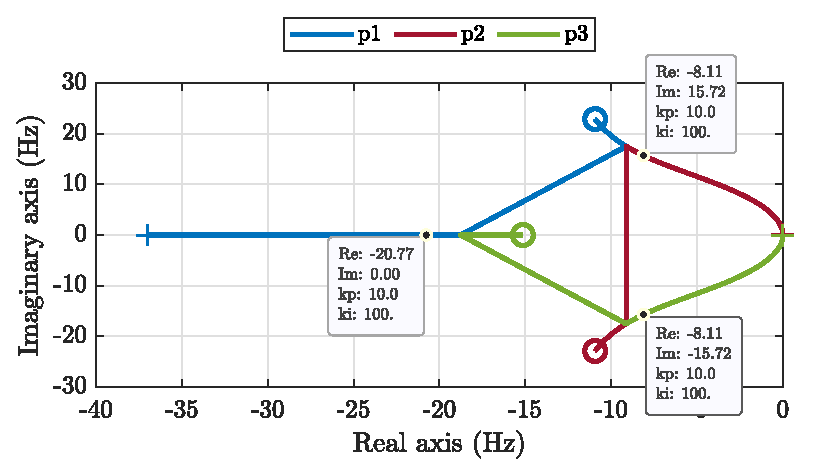
\includegraphics{images/q5_bode_T2.eps}
	\label{fig:q5_bode_a}}
	\hfill
	\subfloat[]{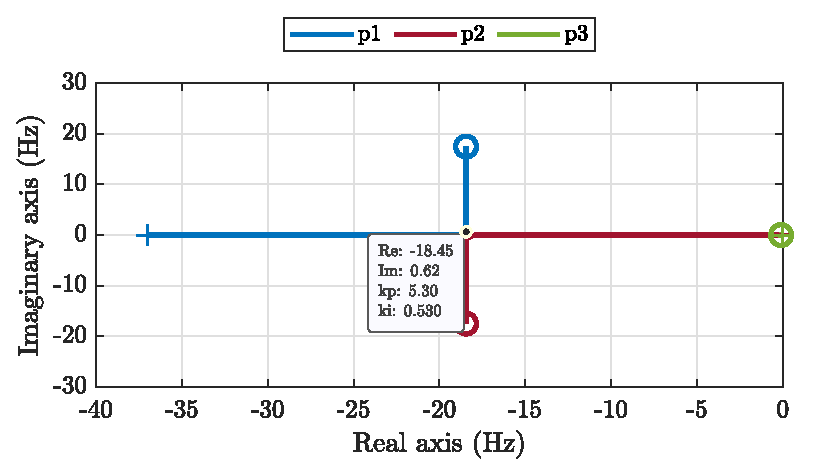
\includegraphics{images/q5_bode_T3.eps}
	\label{fig:q5_bode_b}}
	\caption{Diagram of roots location of close-loop system with proportional-integral control method: (a) $\frac{k_i}{k_p}=10$ and (b) $\frac{k_p}{k_i}=10$.}
	\label{fig:q5_bode_T_PI}
\end{figure}

\begin{figure}
	\centering
	\subfloat[]{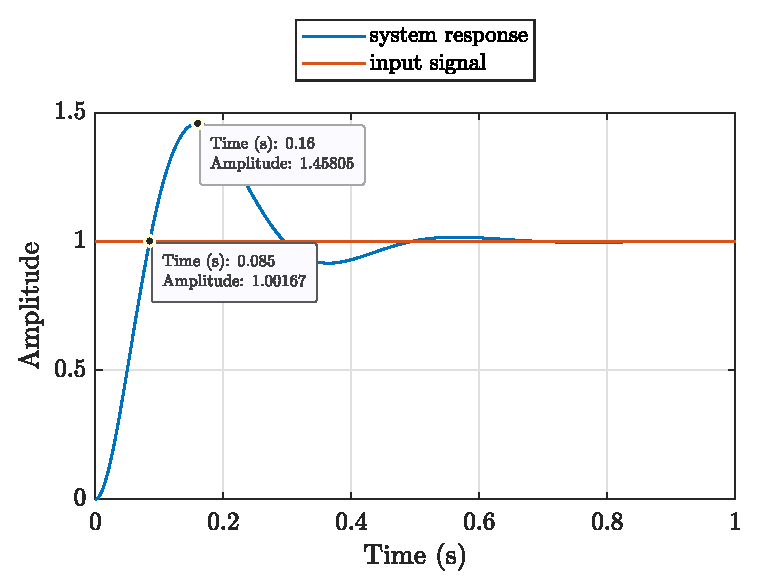
\includegraphics{images/q5_step_response_T2.eps}
		\label{fig:q5_step_a}}
	\hfill
	\subfloat[]{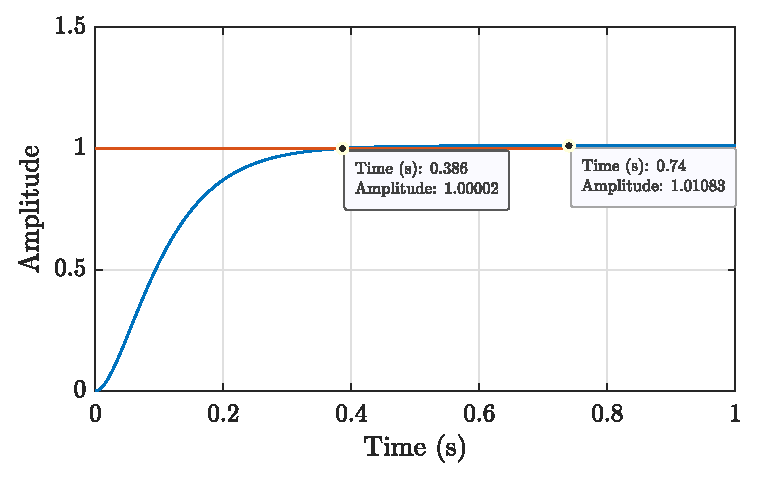
\includegraphics{images/q5_step_response_T3.eps}
		\label{fig:q5_step_b}}
	\caption{Step response of close-loop system with proportional-integral control method: (a) $\frac{k_i}{k_p}=10$ and (b) $\frac{k_p}{k_i}=10$.}
	\label{fig:q5_step_T_PI}
\end{figure}

